\chapter{Introduction to Bessel Functions}
So far we have treated the rectangular waveguide. In this chapter, we will be discussing the circular waveguide. It is a waveguide with circular cross section in the transverse plane whose wave propagates in the z direction. It has metallic walls like a metal pipe and we will understand how waves propagate in this guide. It is useful for making quality cavity resonator (a structure used to store energy). To solve the problem of how wave propagates, we will use the cylindrical coordinates system.

Now the Helmholtz\footnote{Hermann Ludwig Ferdinand Von Helmholtz (31$|$08$|$1821 - 08$|$09$|$1894) was a German physician and physicist who made significant contributions in several scientific fields.}  wave equation:

$$\nabla^2 \bar{E} + h^2 \bar{E} = 0 $$
$$\nabla^2 \bar{H} + h^2 \bar{H} = 0 $$
becomes complex of form shown below for the $E_z$ component of the electric field.
$$\frac{1}{r} \frac{\partial}{\partial r} (r \frac{\partial E_z}{\partial r}) + \frac{1}{r^2} \frac{\partial^2}{\partial \phi ^2}E_z + h^2 E_z = 0 $$
Recall $h^2 = \omega^2 \mu \epsilon + \gamma^2$. This PDE has a solution called the Bessel function. Therefore in this lecture we will introduce the Bessel function.

\section{Bessel Function}
Consider the second order ordinary differential equation (ODE) shown $$x^2 \frac{d^2 y}{dx^2} + x \frac{dy}{dx} + (x^2 - n^2)y = 0$$
The first solution was proposed by Daniel Bernoulli,\footnote{Daniel Bernoulli (8$|$02$|$1700 - 17$|$03$|$1782) was a Swiss mathematician and physicist and was one of many prominent mathematicians in the Bernoulli family, He is particularly remembered for his applications of mathematics to mechanics, especially fluid mechanics, and for his pioneering work in probability and statistics. His name is commemorated in the Bernoulli's principle, a particular example of the conservation of energy, which describes the mathematics of mechanism underlying the operation of two important technologies of the 20th century: the carburetor and the airplane wing.}
from the famous bernoulli principle and it was for analysis for hanging chain (how it oscillates). We all know a pendulum and therefore we have studied its oscillation with a fixed length of chain. However, there is an oscillation when the length is not fixed and that oscillation was described by Daniel Bernoulli. The second solution was by L. Euler\footnote{Leonard Euler (15$|$04$|$1707 - 18$|$09$|$1783) was a Swiss mathematician, physicist, astronomer, logician, and engineer, who made important and influential discoveries in many branches of mathematics, such as infinitesimal calculus and graph theory, while also making pioneering contributions to several branches such as topology and analytic number theory. He also introduced much of the modern mathematical terminology and notation, particularly for mathematical analysis, such as the notion of a mathematical function.} famous for the Euler formula and it was for the theory of vibrations of circular membrane. For instance, the vibrations on a circular drum. In the end, it was Friedrich Bessel (1784-1846)\footnote{Friedrich Wilhelm Bessel (22$|$7$|$784$\rightarrow$17$|$03$|$1846) German Astronomer, mathematician, physicist and geodesist, influenced by Carl Friedrich Wihhelm Argelander. Laplace function was named after him in his death even if originally discovered by Daniel Bernoulli.} who did a systematic study of this PDE and he proposed the various forms of the solution which forms the basis of the Bessel function and the equation above is called the Bessel equation. Bessel functions are probably the next important functions to sines and cosines. They play a role in electromagnetics, Heat transfer, wave motion, elasticity, scattering problems- where waves are scattered from a cylinder or fluids are scattered in a microfluidic channel with cylindrical dimensions. Essentially, any time there is a cylindrical symmetry, the solution is a Bessel function.

From the above Bessel equation written as;
$$x^2 \frac{d^2 y}{dx^2} + x \frac{dy}{dx} + (x^2 - n^2)y = 0$$ \hspace{0.8cm}\text{\parbox{8cm}{n is a real number which is positive or zero.}}

Let's denote $\frac{d^2 y}{dx^2} \equiv y''$ and $\frac{dy}{dx} \equiv y'$

So 
$$x^2y'' + xy' + (x^2 - n^2)y = 0$$
\begin{equation}
x(xy')' + (x^2 - n^2)y = 0
\label{eqn1}
\end{equation} 
  
For a second order PDE we use the series expansion as the solution of the equation which is the Frobenius method\footnote{Ferdinand George Frobenius  (26$|$10$|$1849 - 03$|$08$|$1971) was a German mathematician, best known for his contributions to the theory of elliptic functions, differential equations, number theory, and to group theory. He is known for the famous determinantal identities, known as Frobenius- Stickelberger formulae, governing elliptic functons, and for developing the theory of biquadratic forms.}.

So the proposed solution is 
$$y(x) = \sum_{k=0}^{\infty}C_k x^{K + \alpha} $$
which is a general power series solution; where $\alpha$ is a constant we introduce to the power of x since the power of x may not necessarily be an integer.

Now let's take the derivative of the proposed solution and substitute for the terms $x(xy')'$ and y in equation \ref{eqn1}.

So
$$y' = \sum_{k=0}^{\infty}C_k (k + \alpha) x^{k + \alpha - 1}$$
$$xy' = \sum_{k=0}^{\infty}C_k (k + \alpha) x^{k + \alpha}$$
$$(xy')' = \sum_{k=0}^{\infty}C_k (k + \alpha)^2 x^{k + \alpha - 1}$$
$$x(xy')' = \sum_{k=0}^{\infty}C_k (k + \alpha)^2 x^{k + \alpha}$$
and substituting in equation \ref{eqn1} gives
$$\sum_{k=0}^{\infty}C_k (k + \alpha)^2 x^{k + \alpha} + (x^2 - n^2)\sum_{k=0}^{\infty}C_k x^{k + \alpha} = 0 $$
  
$$\sum_{k=0}^{\infty}C_k (k + \alpha)^2 x^{k + \alpha} - n^2\sum_{k=0}^{\infty}C_k x^{k + \alpha} + \sum_{k=0}^{\infty}C_k x^{k + \alpha + 2} = 0 $$ 

Now we need to determine the various coefficient $C_k$ and the term $\alpha$ we have introduced. The values will be determined by the equation above. First we note that the equation is true for all powers of x i.e for $x^0, x^1 , x^2$ and so on, hence we have a combination of infinite equations. So let us consider the equation for k=0, we have 
$$ C_0 \alpha^2 x^\alpha - n^2C_0 x^\alpha + C_0 x^{\alpha + 2} =0$$ 
Considering the equation for similar exponent of x gives 
$$ C_0 \alpha^2 x^\alpha - n^2C_0 x^\alpha =0$$
$$ C_0 x^\alpha(\alpha^2 -n^2) =0$$
$\Rightarrow C_0 =0$ or $(\alpha^2 -n^2) =0$ 
$$C_0 =0$$ makes no sense, it means the solution is not going to exist so  $$\alpha^2 -n^2 =0$$ or  $$\alpha =\pm n$$

Next let's consider the coefficients of $$x^{\alpha + 1}$$ for k=1
$$C_1(1 + \alpha)^2 x^{1 + \alpha} - n^2 C_1 x^{1 + \alpha} = 0$$
$$C_1x^{1 + \alpha}[(1 + \alpha)^2 - n^2] =0$$
$$C_1x^{1 + \alpha}[1 + \alpha^2 + 2\alpha - n^2] =0$$
Since $$\alpha^2 = n^2$$ then,
$$C_1x^{1 + \alpha}[1 + 2\alpha] =0;$$ for   $$\alpha =\pm n$$
$$C_1x^{1 + \alpha}[1 + 2(\pm n)] = 0$$ which means $$C_1 = 0$$ since $$n \geqq 0$$
Now let's consider the coefficients of $x^{\alpha + 2}$ for k=2 and k=0.
So $$C_2(2 + \alpha) x^{2 + \alpha} - n^2 C_2x^{2 + \alpha} + C_0x^{2 + \alpha} = 0$$
$$C_0 = C_2[n^2 - (2 + \alpha)^2]$$
We can generalize this relationship since a coefficient is always related to 2 coefficient behind, So we have 
$$C_{k-2} = C_k (n^2 - (k + \alpha)^2)$$
Rewriting the expression
$$C_k = \frac{C_{k-2}}{[n^2 - (k + \alpha)^2]}$$
If k is odd for instance k = 3
$$C_3 = \frac{C_{1}}{n^2 - (3 + \alpha)^2} = 0$$ since $C_1 = 0$ 

Also, $C_5$ will be related to $C_3$ and so the odd coefficient does not exist while for k = even, there are even coefficients.
Let $\alpha = \pm n$

So 
$$C_k = \frac{C_{k-2}}{n^2 - (k + n)^2} = \frac{C_{k-2}}{n^2 - k^2 - n^2 - 2nk}$$
$$ =\frac{(-1) C_{k-2}}{k^2 + 2nk} = \frac{(-1) C_{k-2}}{k(2n + k)}$$ where k is even. 
Let $k =2k$ Such that $k = 1, 2, 3, ...$
Then $$C_{2k} = \frac{(-1) C_{2k-2}}{2k(2n + 2k)} = \frac{(-1) C_{2k-2}}{4k(n + k)}$$
for $k=1$
$$C_2 = \frac{(-1) C_0}{4(n + 1)} = \frac{(-1) C_0}{2^2(n + 1)}$$
for $k = 2$
$$C_4 = \frac{(-1) C_2}{2^2 2(2 + n)}$$ and substituting $C_2$ gives 
$$C_4 = \frac{(-1)^2 C_0}{2^4 2(n + 2)(n + 1)}$$
which seems to show a pattern. Now let's find one more term so we can get a generalized relationship.
For k = 3
$$C_6 = \frac{(-1) C_4}{2^2 3(n + 3)} = \frac{(-1)^3 C_0}{2^6 3!(n + 3)(n + 2)(n + 1)}$$	
So, $$ C_{2k} = \frac{(-1)^k C_0}{2^{2k} k!(n + k)(n + k-1)... (n + 1)}$$	

Let's introduce the Gamma Functions to simplify the expression a little further. Gamma function is basically factorial but unlike factorial which works for only integers, it can be done with any number so it is a generalized factorial function. It is given as 
$$\Gamma(n + 1) = n \Gamma(n)$$
So for $$\Gamma(n + 2)$$ it will be expressed as $$\Gamma(n + 2) = (n + 1)\Gamma(n + 1)$$
Same applies for $$\Gamma(n + 3) = (n + 2)\Gamma(n + 2)$$ which can be further simplified by substituting $\Gamma(n + 2)$
So   $$\Gamma(n + 3) = (n + 2)(n + 1)\Gamma(n + 1)$$ and so on.
Now let's consider
$$C_2 = \frac{(-1)^1 C_0}{2^2(n + 1)}$$
which we can rewrite by substituting $ n + 1 = \frac{\Gamma(n + 1)}{\Gamma(n + 2)}$ as 
$$C_2 = \frac{(-1)^1 C_0 \Gamma(n + 1)}{2^2 \Gamma(n + 2)}$$
So the generalized relationship is 
$$C_{2k} =  \frac{(-1)^k C_0 \Gamma(n + 1)}{2^{2k} k! \Gamma(n + k + 1)}$$
Now we can get the series solution for the Bessel Equation for $\alpha= +n$ as 
\begin{dmath*}
y(x) = C_0 x^n \Gamma(n + 1) \left[\frac{1}{\Gamma(n + 1)} - \frac{1}{\Gamma(n+2)}\left(\frac{x}{2}\right)^2 +\frac{1}{2!\Gamma(n+3)}\left(\frac{x}{2}\right)^4 - \frac{1}{3!\Gamma(n+4)}\left(\frac{x}{2}\right)^6 + ... \right]
\end{dmath*}
Let's define $C_0$ as $$\frac{1}{2^n \Gamma(n + 1)}$$ So that
\begin{dmath*}
y(x) = (\frac{x}{2})^n \left[\frac{1}{\Gamma(n + 1)} - \frac{1}{\Gamma(n+2)}\left(\frac{x}{2}\right)^2 +\frac{1}{2!\Gamma(n+3)}\left(\frac{x}{2}\right)^4 - \frac{1}{3!\Gamma(n+4)}\left(\frac{x}{2}\right)^6 + ... \right]
\end{dmath*}
which is called the Bessel function of the first kind. The function has an order of n and it is represented by the term $J_n(x)$
where J is the Bessel function of first kind, n is the order and x is the variable.

We can rewrite the series solution as 
$$J_n(x) = \sum_{k = 0}^{\infty}\frac{(-1)^k (\frac{x}{2})^{2k + n}}{k! \Gamma(n + k + 1)}$$

From ths expression, let's consider the Bessel function for the zeroth order i.e $n=0$
$$J_0(x) = 1 - \frac{(\frac{x}{2})^2 }{1!} + \frac{(\frac{x}{2})^4 }{(2!)^2} - \frac{(\frac{x}{2})^6 }{(3!)^2} + ...$$

if $\alpha = -n,$ then,
\begin{equation}
J_{-n}(x) = \sum_{k = 0}^{\infty}\frac{(-1)^k (\frac{x}{2})^{2k - n}}{k! \Gamma(-n + k + 1)}
\label{eqn2}
\end{equation}
\begin{figure}[h]
\centering
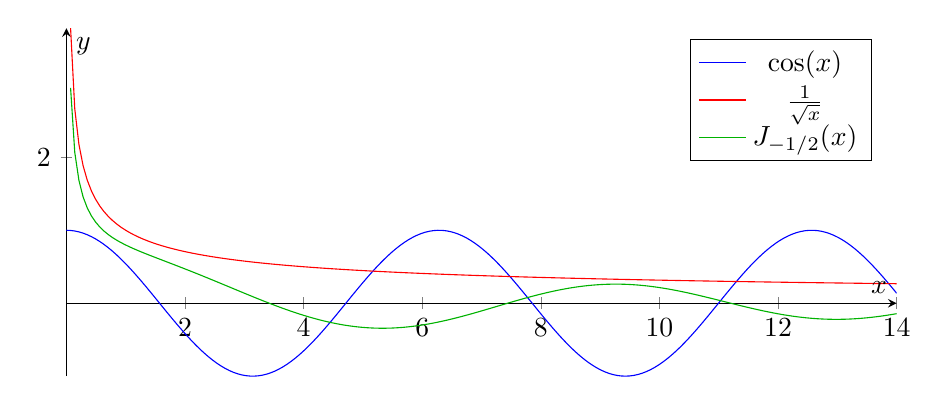
\begin{tikzpicture}
\begin{axis}[
    xlabel=$x$,
    ylabel=$y$,
    domain=0:14,
    samples=200,
    legend pos=north east,
    axis lines=middle,
    width=1\linewidth,
    height=6cm,
]

% Cosine function
\addplot [blue] {cos(deg(x))};
\addlegendentry{$\cos(x)$};

% 1/sqrt(x) function
\addplot [red] {1/sqrt(x)};
\addlegendentry{$\frac{1}{\sqrt{x}}$};

% Bessel function
\addplot [green!70!black] {sqrt(2/(pi*x))*cos(deg(x-sqrt(x)))};
\addlegendentry{$J_{-1/2}(x)$};

\end{axis}
\end{tikzpicture}
\label{fig:fig-1}
\end{figure}
From the plot, it shows that it is the product of $\frac{1}{\sqrt{x}}$ and $\cos(x)$ which are plotted differently. It is seen that at $x=0$, $\frac{1}{\sqrt{x}}$ goes to infinity and as x increases the $\frac{1}{\sqrt{x}}$ term decreases rapidly as shown. The product of the two functions $(\cos(x)$ and $\frac{1}{\sqrt{x}}$) gives the resulting plot of $J_-{\frac{1}{2}}(x)$. It is seen that the zero points are maintained so $J_-{\frac{1}{2}}(x)$ has the periodicity of $\cos(x)$ but the lobes or amplitude of $J_-{\frac{1}{2}}(x)$ goes on decreasing in value as x increases. Below shows the plot of $J_n(x)$ functions
\begin{figure}[h]
\centering
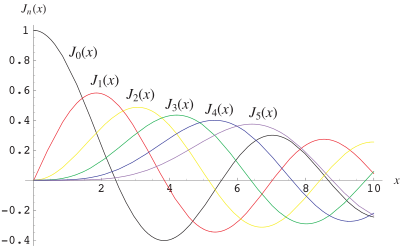
\includegraphics[width=1\linewidth]{./graphics/BesselJ_800}
\caption{Plot of Bessel functions of positive order $J_{n}(x)$}
\label{fig:bessel-functions}
\end{figure}
\begin{figure}[h]
\centering
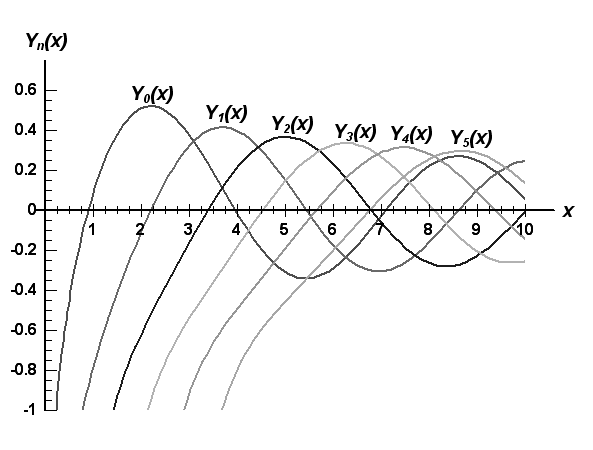
\includegraphics[width=1\linewidth]{./graphics/BesselY_800}
\caption{ Plot of the Neumann functions}
\label{fig:fig-3}
\end{figure}
In general we will have a solution of the form if n is an integer
$$y(x) = AJ_n(x) + B Y_n(x)$$
In the reality, since $Y_n(0) = -\infty$ makes no physical sense in electromagnetics and electrodynamics so the solution will be 
$$y(x) = AJ_n(x)$$
We will stop here for now and consider the circular waveguide in the next lecture. So this lecture was a general introduction to Bessel functions and as electrical engineers these functions play a very important role in cylindrical symmetry. For the metallic waveguide which we will discuss in the next lecture, it is basically the Bessel function of the first kind which is important. When we consider dielectric waveguides such as the optical fibre which will probably be treated in the optical fabrication courses, we will discuss another function called the Hankel function\footnote{Hermam Hankel(14$|$02$|$1839 - 29$|$08$|$1873) German mathematician, he studied and worked with, among others, Mobius, Riemann Weierstrass and Kronecker.} which is the Bessel function of the third kind. It is basically an exponentially decaying function equivalent to the $e^{-\alpha x}$ kind of function for the dielectric waveguide.